\subsection{Rademacher Complexity bound for linear function classes}
In the following section, we will explore a simple exercise for bounding the (Empirical) Rademacher Complexity for linear function classes.

\subsubsection{Problem Statement}
\textbf{Problem} : Let $\F$ be a linear function class defined as followed:
\begin{align*}
    \F = \bigCurl{
        f:\R^d \to \R \Big| f(x) = ax, \|a\|_2 \le R
    }
\end{align*}

\noindent Our objective is to prove the following Rademacher Complexity bound:
\begin{align*}
    \ERC_n(\F) \le \tilde O \bigRound{
        \frac{R}{\sqrt{n}}
    }
\end{align*}

\subsubsection{Covering Number}
\begin{definition}[$\epsilon$-Cover]
    Let $Q$ be a set. $\mathcal{C}$ is called an \textbf{$\epsilon$-cover} of $Q$ with respect to a metric $\rho$ if:
    \begin{align*}
        \forall v \in Q, \exists v'\in \mathcal{C} : \rho(v, v') \le \epsilon
    \end{align*}

    \noindent Basically, $\mathcal{C}$ is an \textbf{$\epsilon$-ball overlapping $Q$}.
\end{definition}

\begin{definition}[Covering Number ($\mathcal{N}(\epsilon, Q, \rho$)]
    The \textbf{covering number} of a set $Q$ is defined as the minimum number of $\epsilon$-covers needed to completely contain $Q$:
    \begin{align*}
        N(\epsilon, Q, \rho) = \text{minimum size of $\epsilon$-covers of $Q$ w.r.t $\rho$}
    \end{align*}

    \noindent Visual illustration of covering number is included in figure \ref{fig:covering_number}.
\end{definition}

\begin{figure}[ht]
    \centering
    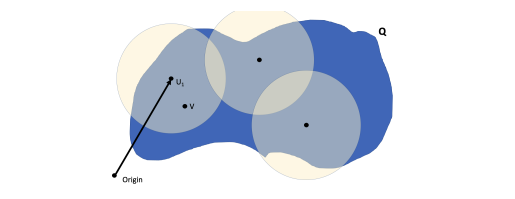
\includegraphics[width=\textwidth]{figures/covering_number.png}
    \caption{Covering number of $Q$ w.r.t a metric $\rho$.}
    \label{fig:covering_number}
\end{figure}

